\section{User Documentation}
\label{sec:userdocs}

This attachment serves as a guided tour of the game and its features.
It is written in such a way that it can be understood even by persons
without a~technical background. These persons may wish to simply
play the game without necessarily developing AI for it, and this attachment
is meant to give them the necessary knowledge.

\subsection{Requirements}

To run \emph{Colonizers}, the Windows 10 operating system is required.
Also required is the following software:
\begin{itemize}
    \item .NET Core 3.1 Runtime
    \item Python 3.7
\end{itemize}

\subsection{Installation}

\emph{Colonizers} is distributed via an installer application, which is shown
in \Cref{ud:installer}.

\begin{figure}[ht]
\centerline{\mbox{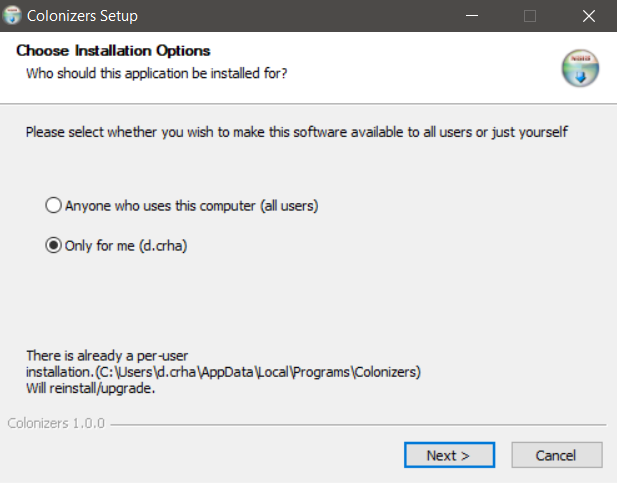
\includegraphics[width=110mm]{installer}}}
\caption{\emph{Colonizers} installer.}\label{ud:installer}
\end{figure}

The installer is an executable named \texttt{Colonizers Setup $x$.$y$.$z$.exe},
where $x$, $y$ and $z$ are placeholders for application versions. During installation,
the user will be asked whether they wish to install the application only for themselves,
or for all users of the computer. We recommend installing the application
only for the current user, since it does not require elevation. The installer
also allows the user to configure the installation directory,
as shown in \Cref{ud:installpath}.

\begin{figure}[ht]
\centerline{\mbox{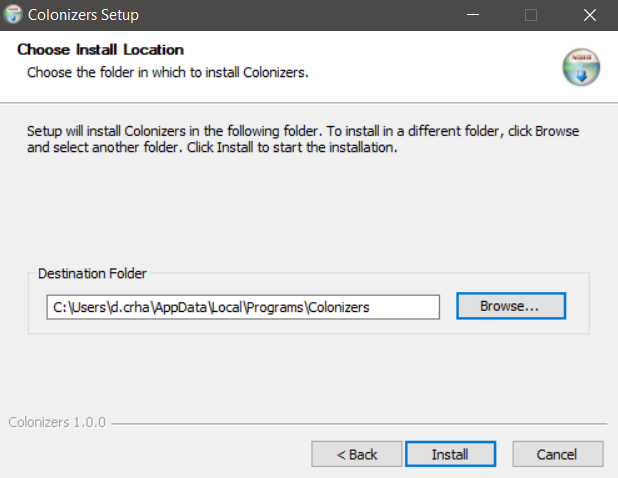
\includegraphics[width=110mm]{installpath}}}
\caption{Choosing the installation path in the installer.}\label{ud:installpath}
\end{figure}

When the installation is finished, the application may be launched from the specified
directory. The installer also adds \emph{Colonizers} into the Start menu, and creates
a~desktop shortcut for the game.

\subsection{Game Configuration}

After launching \emph{Colonizers}, the user will be presented with a~configuration
screen. On this screen, it is possible to configure the game and AI.

The first notable portion of this screen is the player selection, as shown
in \Cref{ud:playerselect}.

\begin{figure}[ht]
\centerline{\mbox{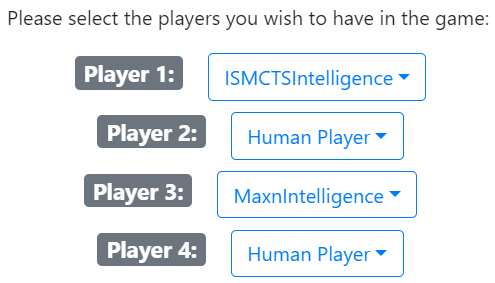
\includegraphics[width=110mm]{playerselect}}}
\caption{Player selection.}\label{ud:playerselect}
\end{figure}

This section contains four dropdowns, each
corresponding to a~player. Each dropdown lists all the available AIs
which are present in the user's game installation. By default, these dropdowns
will have the following values:
\begin{itemize}
    \item \texttt{Human Player}
    \item \texttt{HeuristicIntelligence}
    \item \texttt{ISMCTSIntelligence}
    \item \texttt{MaxnIntelligence}
    \item \texttt{RandomIntelligence}
\end{itemize}
\texttt{Human Player} means that on this player's turn, the UI will become interactible
and the user must choose action to perform. The other player options are AIs which
are bundled with the game. \Cref{ud:aicomp} shows a comparison of the aforementioned
AIs, based on the result of this thesis' experiments. Based on this table,
the user can choose the AI opponents which suit their needs.

\begin{table}[ht]
\centering
\begin{tabular}{l@{\hspace{1.5cm}} c c c c}
\textbf{AI} & \textbf{Strength} & \textbf{Evaluation speed} \\
\midrule
\texttt{RandomIntelligence}      & Weak   & Fast   \\
\texttt{HeuristicIntelligence}   & Moderate   & Fast  \\
\texttt{MaxnIntelligence}        & Moderate   & Moderate  \\
\texttt{ISMCTSIntelligence}      & Strong   & Slow   \\
\bottomrule
\end{tabular}
\caption{Simplified AI comparison.}\label{ud:aicomp}
\end{table}

The next section of configuration is are the buttons for adding new AI
into the game, as shown in \Cref{ud:aiaddbuttons}.

\begin{figure}[ht]
\centerline{\mbox{
\includegraphics[width=110mm]{aiaddbuttons}}}
\caption{Buttons for adding new AI scripts.}\label{ud:aiaddbuttons}
\end{figure}

These buttons open file select dialogs, allowing the user to add new AIs.
When adding an AI script, the script must follow the naming convention
of \texttt{<Name>Intelligence.py}, for example \texttt{CleverIntelligence.py}
\footnote{If an~AI is added this way which shares a~name with and existing AI,
the existing AI will be replaced by the new one. This also applies to AIs which
are bundled with the game}.
If the selected file does not follow this convention, it will not be recognized
by the game.
When adding an AI folder, the folder must follow the naming convention of
\texttt{<Name>Intelligence}, and this foler must contain a \texttt{main.py}
script. If the folder does not follow these conventions, it will not be recognized
by the game. This is explained in more depth in \Cref{chap:aidev}.

Lastly, this screen allows the configuration of the Python executable used
to execute AI scripts, as seen in \Cref{ud:pythonselect}. The shown
button will open a file select dialog, where the user can select their
installed Python executable.

\begin{figure}[ht]
\centerline{\mbox{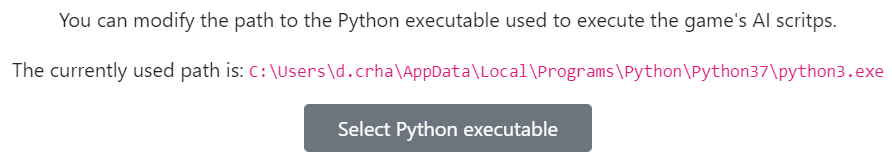
\includegraphics[width=110mm]{pythonselect}}}
\caption{Configuration of Python executable.}\label{ud:pythonselect}
\end{figure}

After the user is done configuring the game, they may start a game by clicking the
\emph{START GAME} button. Note that this button is disabled if the user
has not specified a Python executable to use.

\subsection{Gameplay}

WORK IN PROGRESS
